In diesem Kapitel werden die Datenstrukturen und Algorithmen des neuen im
Rahmen der Diplomarbeit entwickelten ringmap-Packet-Capturing-Stack für
Betriebssystem FreeBSD dargestellt. Das Ziel des Entwurfes war einen neuen
Capturing-Stack mit verbesserter Performance zu erarbeiten. Dafür wurden
durch Analyse im Kapitel \ref{sec:aufgstel} die Probleme des aktuellen
generic-Capturing-Stack herausgestellt. Anhand der gefundenen Probleme
wurden die Anforderungen für den neuen ringmap-Stack, mit dem Ziel den
Datendurchstz beim Capturing zu erhöhen, erstellt.\\\\
%
\subsection{Datenstrukturen}
Die im \emph{ringmap}-Capturing-Stack verwendete Daten-Strukturen dienen zur Modellierung
aller für Paketempfang verantwortlichen Paket-Puffer in Form  eines
Ringpuffers. Die Gründe für die Auswahl der Ringpuffer-Struktur sind in
folgenden Abschnitten dargestellt. Der Stacks sind für die
Paketzustellung und den Paketzugriff im Ringpuffer und auch für die Steuerung
des Capturing-Prozesses zuständig.

\subsubsection{Verwendungszwecke für Ringpuffer}
Die Ringpuffer-Daten-Struktur wird bevorzugt wenn es um den Datenzugriff in
einem Array oder einer Liste handelt, bei der die Elementenanzahl konstant bleiben
soll und neue Speicherallozierungen unerwünscht wären. Darüberhinaus werden
Ringpuffer für die Lösung einiger klassischen Problemen, z.B.
Erzeuger-Verbraucher-Problem~\cite{erz_verbr_wiki},
empfohlen~\cite{ldd_book_circle_buffer}.

\subsubsection{Gründe für die Ringpuffer-Struktur im ringmap-Capturing-Stack}
Die Gründe für die Auswahl der Ringpuffer-Struktur für den Paket-Capturing
basieren vor allem auf den im Kapitel \ref{sec:aufgstel} für den 
\emph{ringmap}-Capturing-Stack gestellten Anforderungen (Anforderungen \textbf{1.} und
\textbf{2.}). Außerdem spielen für die Auswahl der Ringstruktur auch die
andere folgende Faktoren und die Hardware-Eigenschaften eine wichtige Role:
\begin{itemize}
	\item Der Capturing-Prozess ist dem
		Erzeuger-Verbraucher-Modell~\cite{erz_verbr_wiki} ähnlich:
		\begin{itemize}
			\item Es gibt ein ``Datenerzeuger'': der Netzwerkadapter-Treiber, der die
				Pakete in den Ringpuffer für folgende Bearbeitung bzw.
				Filterung vorbereitet.
			\item Es gibt  ein ``Datenverbraucher'': die User-Anwendung, die
				auf die in den Paket-Puffer befindlichen Pakete zugreift,
				sie bearbeitet, speichert oder darstellt.
		\end{itemize}
	\item Der Netzwerkadapter verwaltet die Deskriptoren als ein Ringpuffer (siehe
		Abschnitt \ref{sec:adapter}).  Der Netzwerkadapter enthält die
		\verb+RDT+- und \verb+RDH+-Register, welche die Role der HEAD und
		TAIL-Pointers im Deskriptor-Ringpuffer speilen und dadurch, dass jeder
		Deskriptor einen Paket-Puffer referenziert, können diese Register auch
		als HEAD und TAIL für den Paket-Puffer-Array nützlich sein.
\end{itemize}

\subsubsection{Memory-mapped Paket-Ringpuffer für ringmap-Capturing-Stack}\label{sec:memmap_pr}
Alle Paket-Puffer werden in den Adressraum eines Capturing-Prozesses
eingeblendet, damit der Capturing-Prozess ohne Kopie-Operationen und ohne
Systemaufruf auf die Pakete zugreifen kann. Mit jedem Paket-Puffer werden zwei
weitere Daten-Strukturen in den Userspace eingeblendet. Das sind
\verb+mbuf+~\cite{man_bpf} und Deskriptor.  Diese Strukturen werden im Userspace
deshalb gebraucht, weil sie die für Paketbearbeitung und Paketfilterung
relevante Informationen enthalten.  Auf diese obengenannten Datenstrukturen
wird sowohl vom Kernelspace als auch vom Userspace zugegriffen.  Um dies zu
ermöglichen werden drei andere Datenstrukturen zur Adressierung vorgesehen, 
welche sowohl die Kernelspace- als auch die Userspace-Adressen von den 
Paket-Puffer, \verb+mbuf+'s und Deskriptoren enthalten.
Das sind: \verb+PAKET+, \verb+MBUF+ und  \verb+DESKRIPTOR+ (siehe Abbildung
\ref{img:uml_ring}).\\\\
%
Jedes Paket im RAM wird durch den Tripel \verb+[PAKET, MBUF, DESKRIPTOR]+
repräsentiert. Jedes Tripel wird in einer Datenstruktur \verb+RING_SLOT+
gekapselt.  Und die Instanzen von \verb+RING_SLOT+ bilden ein Array,
der in der \verb+RING+-Struktur enthalten ist.  Die \verb+RING_SLOT+-Struktur
enthält unter anderem die Platzhalter für \verb+Timestamp+ und \verb+Counter+
vom repräsentierten Paket.\\\\
%
\verb+RING+-Struktur enthält den Array von \verb+RING_SLOT+-Instanzen und die
\verb+HEAD-+ und \verb+TAIL+-Pointers, welche die \verb+HEAD-+ und
\verb+TAIL-+Slots im \verb+RING_SLOT+-Array referenzieren. Damit bildet
\verb+RING+ eine Datenstruktur die es erlaubt, alle  Paket-Puffer als ein
Ringpuffer zu betreiben.\\\\
%
Die \verb+RING+-Struktur wird mit den Paket-Puffer in den Adressraum eines
Userspace-Capturing-Prozesses eingeblendet, und erlaubt ihm den Zugriff auf alle
Paket-Puffer und das Betreiben aller Paket-Puffer als ein Ringpuffer.
%
\begin{figure}
\centering 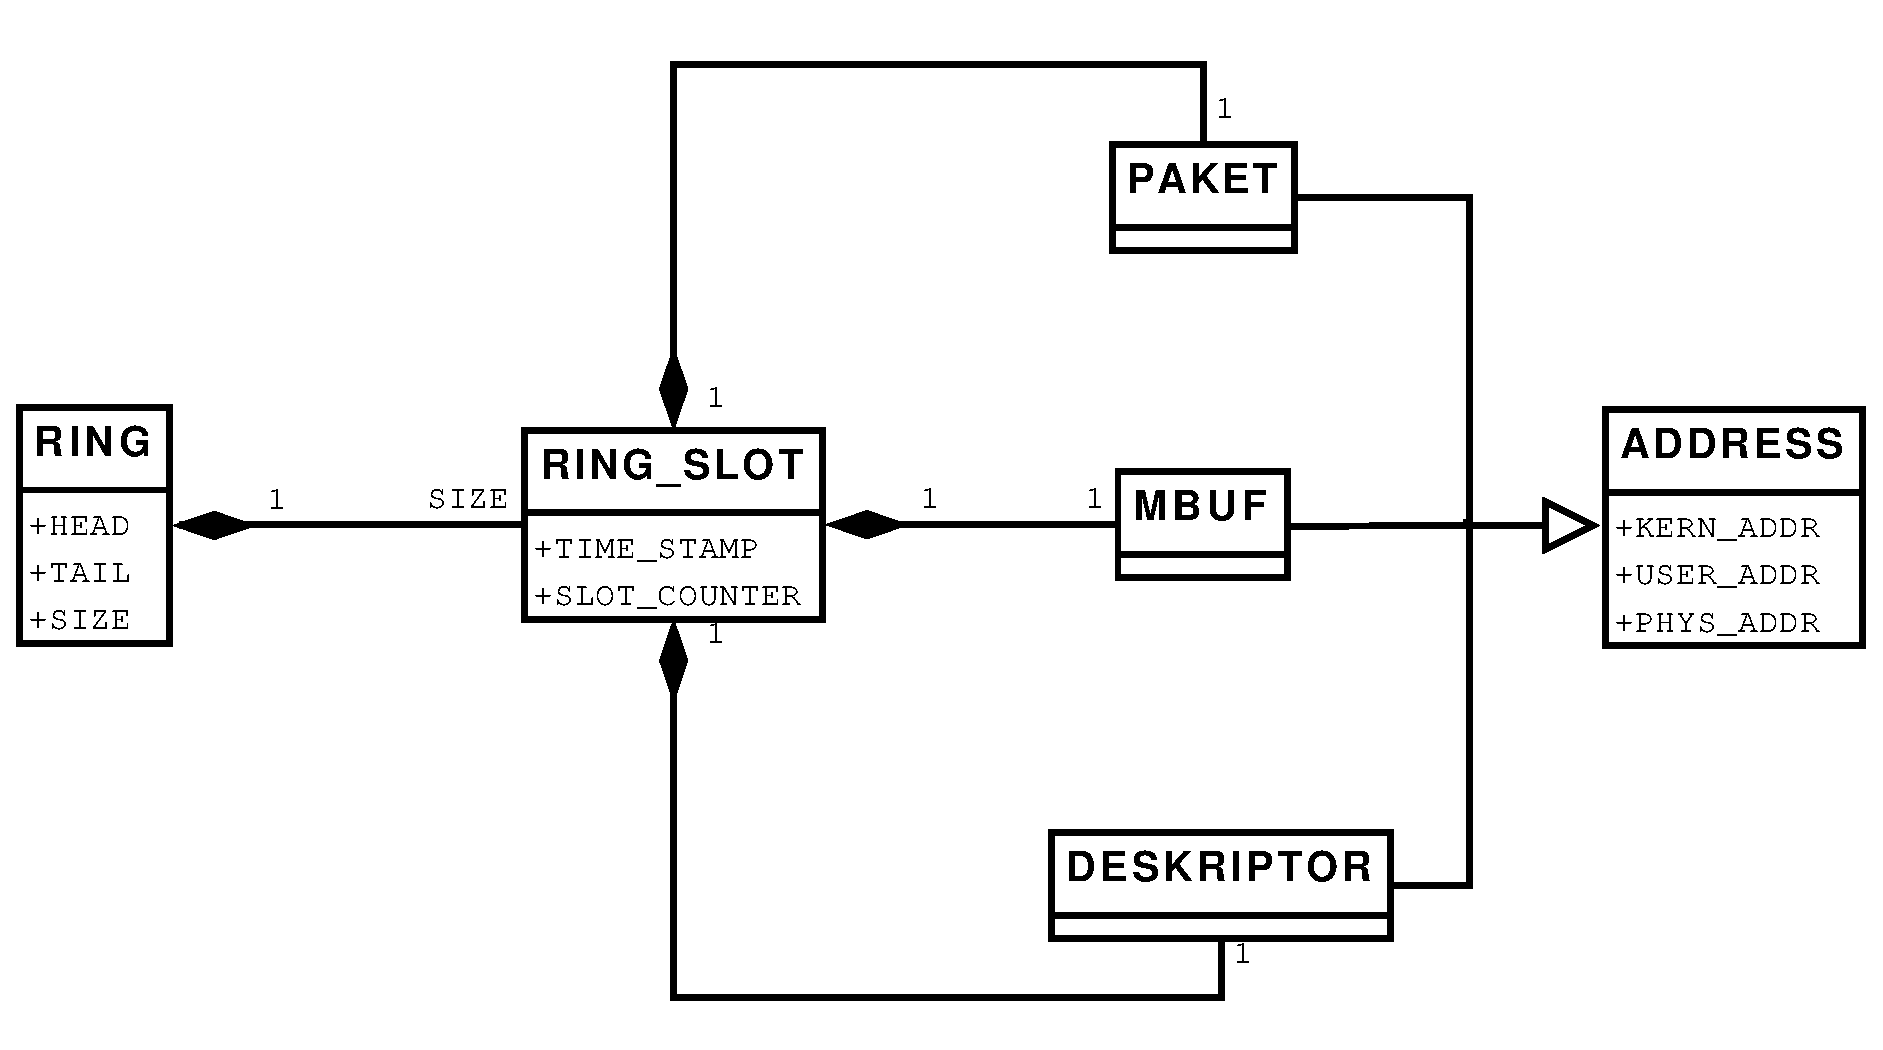
\includegraphics[width=6.4in]{bilder/uml_RING_Puffer}
\caption{Datenstrukturen des Ringpuffer}
\label{img:uml_ring}
\end{figure}

\newpage
\subsection{Funktionalität}
Der neue Capturing-Stack enthält die folgende Funktionalitäten:
\begin{itemize}
	\item \textbf{Paketzustellung}:
		\begin{itemize}
			\item Zustellung der Pakete in den Ringpuffer wird mit Hilfe des
				\textbf{Netzwerkadapter-Treibers} realisiert. 
		\end{itemize}
	\item \textbf{Paketzugriff}:
		\begin{itemize}
			\item  Zugriff auf die im Ringpuffer befindlichen Pakete  wird beim
				\textbf{Userspace-Capturing-Prozesses} gemacht.
		\end{itemize}
	\item \textbf{Systemaufrufe} für:
		\begin{itemize}
			\item Memory-Mapping.
			\item Capturing-Steuerung:  Capturing-Anhalten und -Fortsetzen.
			\item Blockierendes Warten auf neue Pakete.
		\end{itemize}
	\end{itemize}
Aufgrund der Anforderung 4. (siehe Kapitel \ref{sec:aufgstel}), darf
in einem Capturing-Stack nur ein Paketzugriff-Prozess sein. Weil es  nur einen
Zustellung-Prozess (den Treiber) und nur einen Paketzugriff-Prozess gibt,
werden keine \emph{race conditions} beim Zugriff auf Paket-Puffer auftreten,
und dadurch werden keine Synchronisation-Maßnahmen benötigt ~\cite{ldd_book_circle_buffer}.\\\\
%
Nach der Anforderung 3. dürfen während des Ablaufs des Capturing keine
Systemaufrufe auftreten. Gemeint sind die Systemaufrufe die für den Zugriff auf
empfangene Pakete gebraucht wären. Durch \textbf{Memory-Mapping} werden die
Systemaufrufe für den Paketzugriff eliminiert. Es gibt aber die Systemaufrufe
die nicht zu beseitigen sind. Das sind die, welche für die Realisierung vom
\textbf{Memory-Mapping} selbst benötigt werden.  Außerdem wurden auch die Systemaufrufe
für die \textbf{Capturing-Steuerung} und \textbf{blockierendes Warten} auf neue
Pakete implementiert. Theoretisch könnte man die \textbf{Capturing-Steuerung}
durch die Interaktion mit dem Kernelspace über die eingeblendete
Speicherbereiche realisieren. Das \textbf{blockierende Warten} ist auch nicht
die einzige Lösung, wenn der Userspace-Prozess auf die neue Pakete warten soll.
Er kann ja auch aktiv, in einer Schleife, warten.  Das Vermeiden von
Systemaufrufen für die zwei obengenannten Probleme (Capturing-Steuerung und
blockierendes Warten) ist zwar losbar, hat aber einen zusätzlichen Aufwand und
stellt den Performance-Gewinn unter die Frage:
\begin{itemize}
	\item \textbf{Capturing-Steuerung über Shared-Memory}: Wenn der
		Capturing-Prozess nicht über den Systemaufruf, sondern über die
		\emph{Shared-Memory} eine Anfrage an Treiber stellt, soll er darauf
		warten, bis der Treiber-Prozess die CPU für seinen Ablauf bekommt.  Da
		die Funktionen des Treibers, die nicht in folge eines  Systemaufrufes,
		sondern in folge eines  Interrupts aufgerufen werden, in den
		unvorhersagbaren Zeitpunkten stattfinden, kann es dazu führen, dass der
		Capturing-Prozess keine sofortige Reaktion vom Treiber nach seiner
		Anfrage bekommt. Dieses Problem kann mit Hilfe eines
		Kernel-\emph{Watchdog}~\cite{wiki_watchdog} gelost werden, was aber
		nicht nur einen Implementierung-Aufwand mit sich bringt, sondern auch
		den Systemload erhöht.
	\item \textbf{Das aktive Warten auf die neue Pakete}: Das aktive Warten
		beansprucht keinen Systemaufruf dennoch vermeidet das keinen
		Kontextwechsel-Overhead, denn das Betriebssystem blockiert selber im
		Lauf des Prozess-Scheduling den laufenden Prozess um den anderen
		Prozessen die CPU zur Verfügung zu stellen. Außerdem reduziert das
		Betriebssystem die Priorität des aktiv wartenden Prozesses wegen seiner
		ständigen CPU-Nutzung, was die Capturing-Performance negativ
		beeinflussen kann.
\end{itemize}
Jeder Systemaufruf bringt unvermeidlich mit sich einen Overhead (Kontextwechsel
und ggf. Daten-Kopieren) mit sich. Wie kritisch dieser Overhead für
Capturing-Performance ist, hangt von der Häufigkeit des Auftretens der
Situationen, in denen die Systemaufrufe gebraucht werden.  Das
\textbf{Memory-Mapping} im FreeBSD kann nur mit Hilfe eines Systemaufrufes in
die Tat gebracht werden, deshalb für dieses Vorgehen ist der Systemaufruf nicht
zu vermeiden. Die \textbf{Capturing-Steuerung} ist eher ein seltenes Ereignis,
denn es wird ja nicht ständig gebraucht, softwaremässig den Capturing
anzuhalten und fortzusetzen.  Deshalb ist die Verwendung der Systemaufrufen für
Capturing-Steuerung eher unkritisch. Wenn es aber um Warten auf neue Pakete
geht, dann ist aufgrund der unvorhersagbaren Netz-Verkehr das Auftreten des
wartendes Zustandes auch nicht berechenbar ist. Dennoch für das Warten auf neue 
Pakete wird in \emph{ringmap} blockierendes Warten verwendet.
%
In den folgenden Abschnitten werden die Algorithmen der im Capturing-Stack 
beteiligten Funktionalitäten dargestellt.

\subsubsection{Paketzustellung in den Ringpuffer. Netzwerktreiber}
Die Paket-Zustellung in den Ringpuffer wird beim Netzwerkadapter-Treiber
erledigt. Die eigentliche Zustellung macht natürlich der Adapter durch den
DMA-Transfer selbst.  Der Treiber bereitet nur die in den RAM geschriebene
Daten für die weitere Bearbeitung und den Zugriff auf ihnen.  Da aus dem Sicht
des Userspace-Prozesses, der auf die empfangene Pakete zugreift, die
Hardware-Funktionalität unsichtbar ist, spielt der Treiber die Rolle des
Paket-Zusteller.\\\\
%
Die folgende Beschreibung von der Funktionalität des neuen im Rahmen der
Diplomarbeit implementierten \emph{ringmap}-Netzwerkadapter-Treiber trennen wir auf zwei logischen
Teile. Das sind: \textbf{Treiber-Initialisierung} und
\textbf{Capturing-Ablauf}.\\\\ 
%
Bei \textbf{Treiber-Initialisierung} werden alle für Capturing benötigte Speicherbereiche 
(Paket-Puffer, Deskriptoren, etc\ldots) alloziert und initialisiert.\\\\
%
Während des \textbf{Ablauf} von Capturing bestehen die Aufgaben vom Treiber
darin, jeden neuen in den RAM geschriebenen Puffer zu ``checken'', TAIL- und
HEAD-Pointer mit den RDH- und RDT-Register zu synchronisieren und den für die
neue Pakete wartenden Userspace-Capturing-Prozess ausblockieren.

\subsubsection*{Treiber-Initialisierung} 
\begin{figure}
\centering 
\includegraphics[width=3.9in]{bilder/FlowChart_Treiber_Init}
\caption{Treiber: Initialisierung}
\label{img:new_treiber_init}
\end{figure}
Die Initialisierungsfunktionen von Treiber werden beim Laden des Treibers
ausgeführt.  In Abbildung \ref{img:new_treiber_init} ist der Flow-Chart-Diagram
des Initialisierung-Prozesses dargestellt. Folgend beschreiben wir den den auf
dem Diagram dargestellten Algorithmus.
\begin{enumerate}
	\item Es wird den Speicher für \verb+RING+-Struktur alloziert.
	\item Der Speicher für alle Deskriptoren wird alloziert. Die physische
		Adresse des ersten Elementes von Deskriptor-Array wird in ein Register
		des Netzwerkadapters gesetzt, um dem Netzwerkadapter den Zugriff auf
		Deskriptoren zu ermöglichen~\cite{e1000_sdm}.
	\item Der Speicher für Paket-Puffer wird alloziert.
	\item Die physische Adresse des allozierten Paket-Puffer wird in den 
		\verb+Address+-Feld des Deskriptors geschrieben (siehe Abbildung
		\ref{dma-e1000-desc}). 
	\item Wiederhole die Schritte \textbf{3.} und \textbf{4.} für alle 
		\verb+RING+-Slots (bzw. Deskriptoren).
\end{enumerate}
Nach der Initialisierung-Phase des Treibers sind die Deskriptoren
kontinuierlich  im physischen Speicher alloziert und initialisiert. Darüber
hinaus sind die Paket-Puffer alloziert und die physische Adressen von den
Paket-Puffer sind in den \verb+Address+-Felder der Deskriptoren gesetzt (siehe
Abbildung \ref{dma-e1000-desc}). Nach dem setzen der physischen Adresse des 
ersten Deskriptor in den \verb+RDBAL+- und \verb+RDBAH+-Adapter-Register, 
kann der Netzwerkadaptern mit dem Capturing anfangen.

\subsubsection*{Ablauf des Capturing}\label{sec:new_treiber_ablauf}
Die \emph{Flow-Chart}-Diagram des Kernel-Threads ist in Abbildung
\ref{img:new_kernel_thread} dargestellt. Der Kernel-Thread bearbeitet maximal
\verb+rx_processing_limit+ Slots und beginnt mit dem Slot, dessen Nummer in der globalen
\verb+current_SLOT+-Variable gespeichert ist. Die Variable \verb+current_SLOT+ 
wird nach der Bearbeitung jedes Ringslots inkrementiert, sodass sie 
der Nummer des nächsten Slot im Ringpuffer entspricht.\\\\
Folgend beschreiben wir den Algorithmus  des neuen Kernel-Threads: 
\begin{enumerate}
	\item Speichern des \verb+RING.TAIL+-Wertes in RDT-Register 
		\begin{itemize}
			\item Der Userspace-Process soll nach dem Zugriff auf Paket den Wert
				\verb+RING.TAIL+ so erhöhen, dass \verb+RING.TAIL+ der
				Nummer des zuletzt gelesenen Slots entspricht.
			\item Der Kernel-Thread setzt \verb+RING.TAIL+-Wert in 
				RDT-Register und übergibt damit dem  Netzwerkadapter die neue freie
				Deskriptoren für den DMA-Transfer der nächsten Pakete (siehe
				Abschnitt \ref{sec:hw_dma}). 
		\end{itemize}
	\item Berechnen der Verkehrsstatistiken. 
		\begin{itemize}
			\item \emph{Time-Stamp} wird berechnet und in \verb+SLOT+-Struktur gesetzt.
		\end{itemize}
	\item \verb+current_SLOT+ \emph{modulo} \verb+RING.SIZE+ inkrementieren.
		\begin{itemize}
			\item \verb+current_SLOT+ ist dann die Nummer des nächsten 
				für Bearbeitung stehenden Slot.
		\end{itemize}
	\item  Der wert von \verb+current_SLOT+ wird in \verb+RING.HEAD+ gesetzt. 
		\begin{itemize}
			\item Damit wird für den  Userspace-Prozess noch ein Slot zur Verfügung
				gestellt.  Die Slots von \verb-RING.TAIL + 1- bis zu dem Slot
				mit der Nummer \verb+RING.HEAD - 1+ enthalten die neue Pakete,
				welche der Userspace-Prozess noch bearbeiten soll (siehe
				Abschnitt \ref{sec:hw_dma}). 
		\end{itemize}
	\item \verb+count+ wird dekrementiert.
	\item Der wartende Userspace-Capturing-Prozess wird ausblockiert wenn 
		der Kernel-Thread alle \verb+rx_processing_limit+ Paket-Puffer
		oder alle neue nach dem letzten Interrupt im RAM befindlichen Paket-Puffer 
		bearbeitet hat.
\end{enumerate}
%
\begin{figure}
\centering 
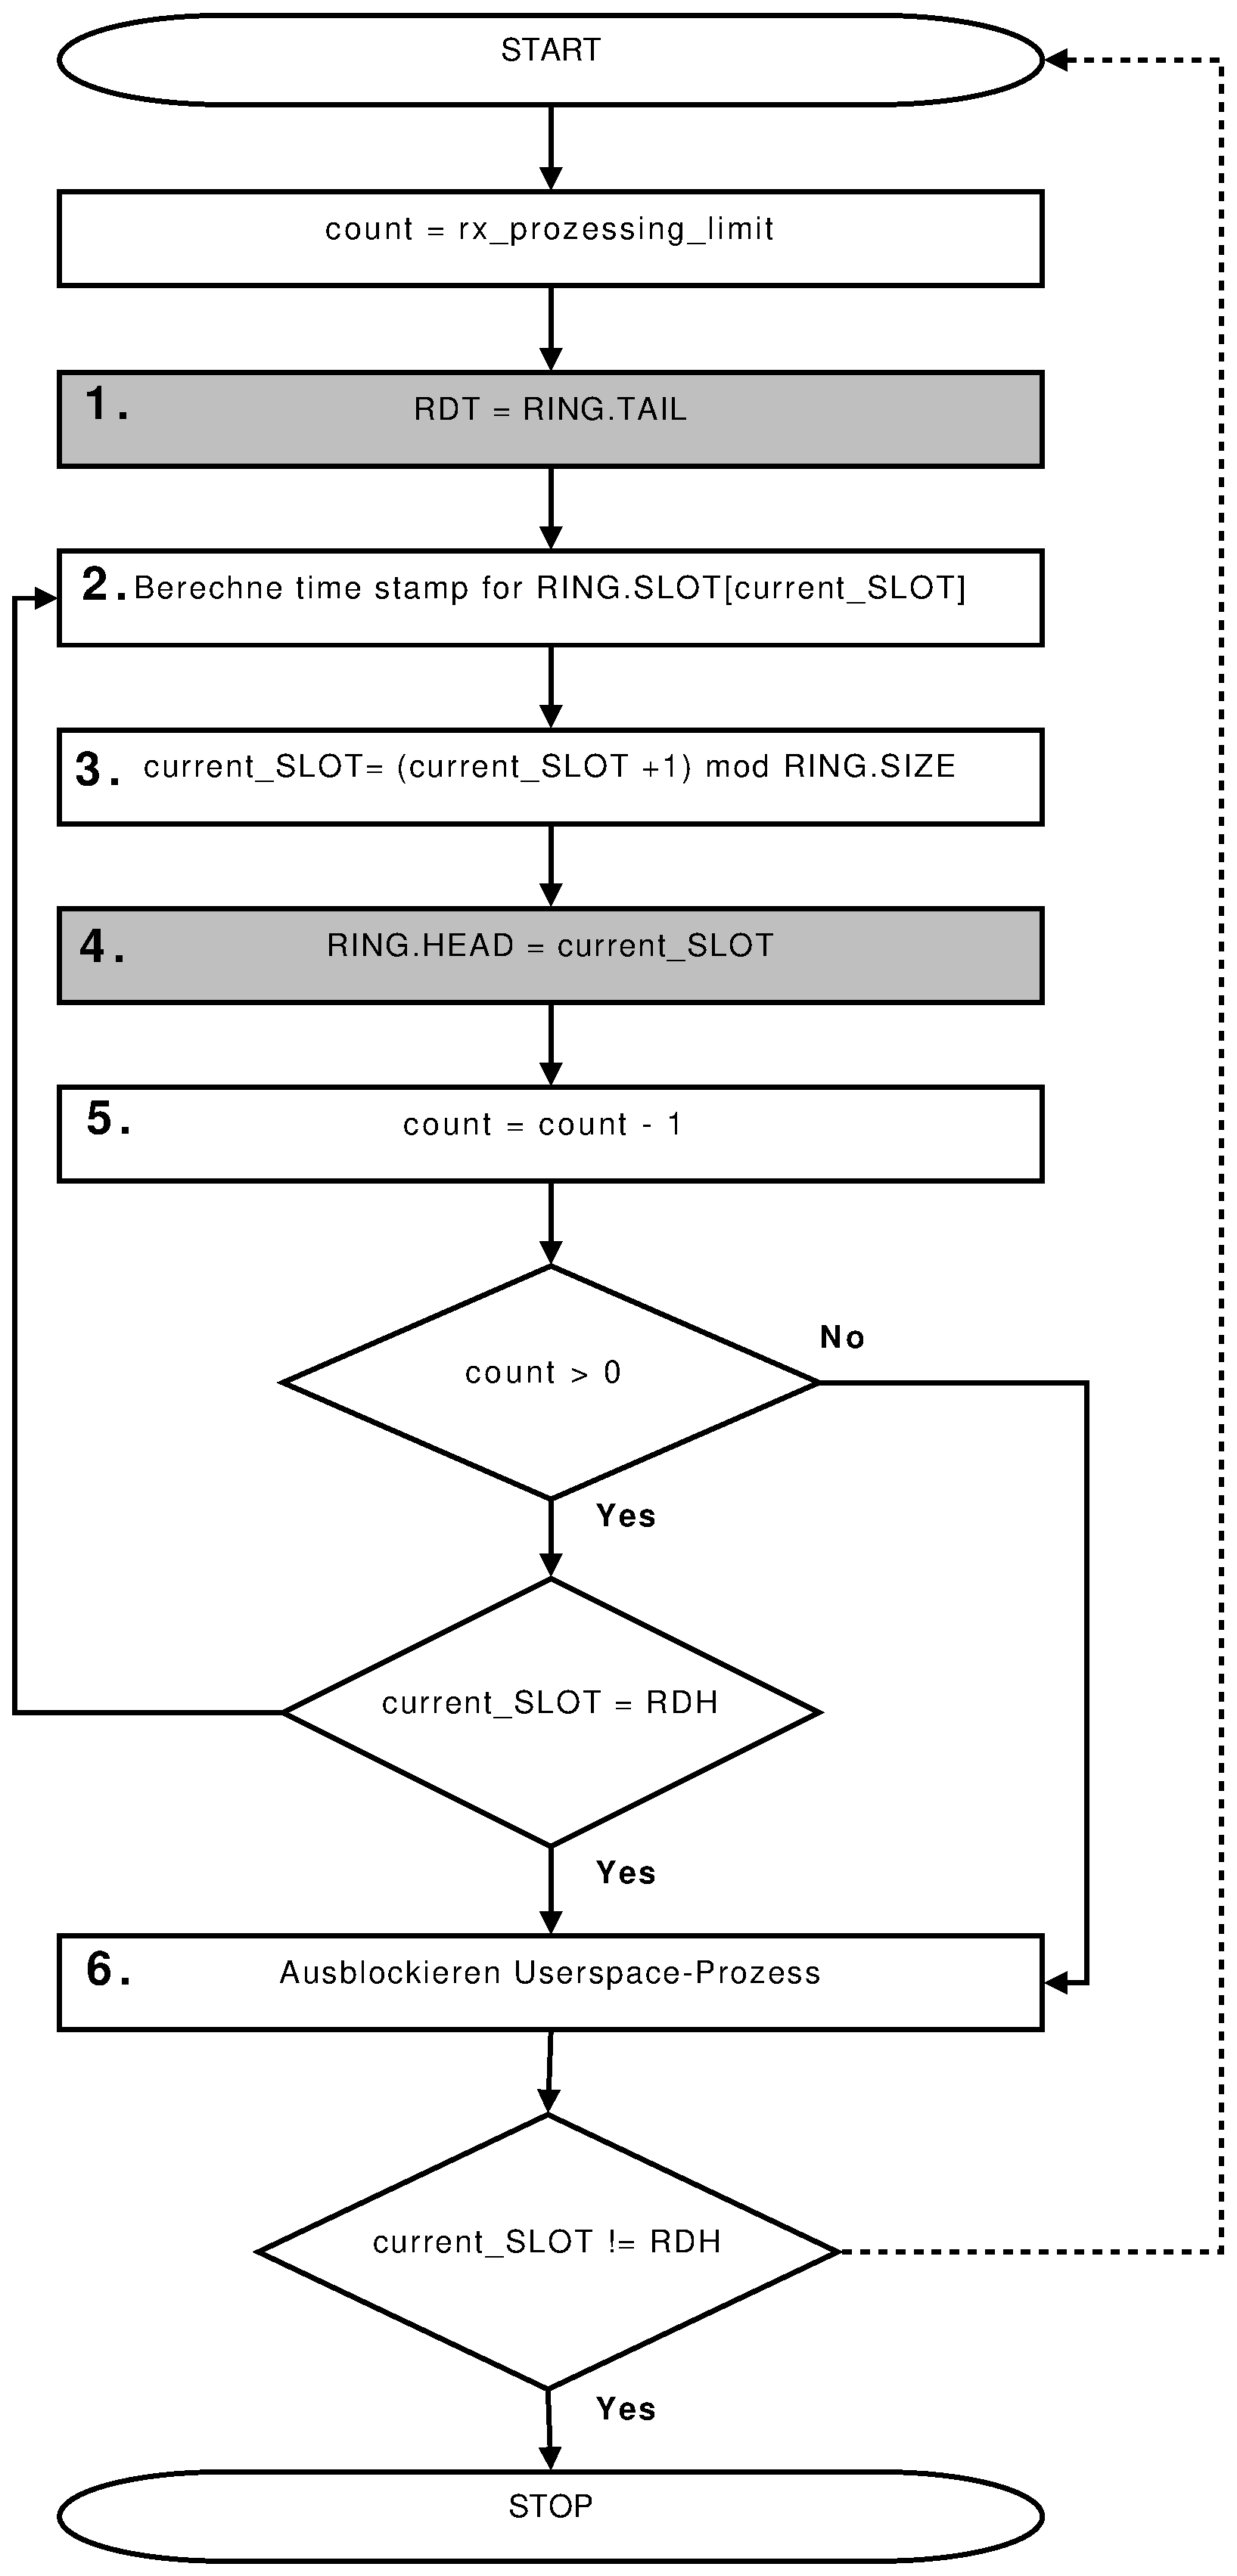
\includegraphics[width=4.2in]{bilder/FlowChart_New_Kernel_Thread}
\caption{Capturing-Ablauf. Kernel-Thread des \emph{ringmap}-Netzwerkadapter-Treibers}
\label{img:new_kernel_thread}
\end{figure}
Die graugezeichneten Boxen in Abbildung \ref{img:new_kernel_thread} bezeichnen
die Operationen, die zur Verwaltung von den \verb+TAIL+- und
\verb+HEAD+-Ringpointers dienen.  Dadurch, dass die \verb+RING+-Struktur in den
Userspace eingeblendet ist und damit sowohl im Userspace als auch im
Kernelspace zur Verfügung steht, können der Treiber und der Userspace-Prozess
durch das Setzen von \verb+RING.TAIL+- und \verb+RING.HEAD+-Pointers einander über
die gemachte Arbeit benachrichtigen. \\\\
%
Der Userspace-Prozess liest die neue
Paket-Puffer bis zu dem Paket-Puffer mit der Nummer \verb+RING.HEAD - 1+, und
wird blockiert für das Warten auf neue Pakete. Nach jeder Bearbeiten des neuen
Paket-Puffer setzt der Userspace-Prozess in \verb+RING.TAIL+ die Nummer der
gerade gelesenen Slot, und sobald der Kernel-Thread an der Reihe ist, liest der
Kernal-Tread diesen Wert und setzt ihn in  RDT-Register.\\\\
%
Der Netzwerkadapter-Treiber beschreibt die Paket-Puffer mit den neuen Daten beginnend
von dem Slot, desser Nummer im \verb+RDH+-Register bis zu dem Slot desser
Nummer im \verb+RDT+-Register gespeichert ist, und damit überschreibt nicht die
Paket-Puffer die von dem Userspace-Prozess noch nicht bearbeitet wurden.

\subsubsection{Systemaufruf-Funktionen}\label{sec:entw_syscalls}
Die Systemaufrufe sind dazu gebraucht werden, um dem Interaktion zwischen den
Netzwerkadapter-Treiber und Userspace-Capturing-Prozess zu ermöglichen. Dabei werden
dem Userspace-Prozess die Funktionen zur Verfügung zu gestellt, die er aufgrund
der Hardwarebegrenzungen nicht selber ausführen kann.\\\\ 
%
Die Systemaufrufe werden in unserem \emph{ringmap}-Capturing-Stack für die folgende
Zwecke gebraucht: 
\begin{itemize}
	\item Capturing-Steuerung
		\begin{itemize}
			\item Anhalten und Fortsetzen des Paketempfangs beim Netzwerkadapter
		\end{itemize}
	\item Memory-Mapping
		\begin{itemize}
			\item Allozieren und Initialisieren der \verb+RING+-Struktur (siehe
				Abbildung \ref{img:uml_ring}).
			\item Liefern dem Userspace-Prozess der physischen Adresse der
				\verb+RING+-Struktur.
			\item Das eigentliche \emph{Memory-Mapping} wird vom
				Userspace-Prozess durch den \emph{mmap}-Systemaufruf auf dem
				device \verb+/dev/mem+ realisiert.
		\end{itemize}
	\item Blockierendes Warten auf neue Pakete
		\begin{itemize}
			\item Sobald keine neue Pakete zur Bearbeitung für den
				Userspace-Prozess im RAM liegen wird der Userspace-Prozess
				blockiert und erst nach dem Ankommen der neuen Pakete
				durch den Kernel-Thread wieder ausblockiert (siehe Abschnitt
				\ref{sec:new_treiber_ablauf}, Abbildung
				\ref{img:new_kernel_thread})
		\end{itemize}
\end{itemize}
\subsubsection*{Capturing-Steuerung}
Capturing-Steuerung wird mit Hilfe des \emph{ioctl}-Systemaufrufes realisiert.
Die primäre Aufgaben dabei sind \emph{Capturing-Anhalten} und
\emph{Capturing-Fortsetzen}.  Die Idee liegt daran, dass der Userspace-Prozess
einen \emph{ioctl}-Systemaufruf macht, dann wird die für den Aufruf
verantwortliche Funktion im Kernelspace ausgeführt, welche über die Beschreiben
des Control-Register des Netzwerkadapters den Paketempfang anhält oder
fortsetzt.\\\\ 
%
Die Details sind im Kapitel \textbf{Implementierung} im Abschnitt
\ref{sec:impl_treiber} beschrieben.
 
\subsubsection*{Memory-Mapping}\label{sec:memmap}
Die Memory-Mapping wird mit dem \emph{mmap}-Systemaufruf auf dem Device
\verb+/dev/mem+ realisiert. Als Argument bekommt der \emph{mmap} die physische
Adresse und die Byte-Länge des Speicherbereiches, der in den Userspace
eingeblendet wird, und liefert dem Userspace-Prozess die gültige
Userspace-Adresse des eingeblendeten Speicher-Bereich zurück.\\\\
%
Das heißt, der Userspace-Capturing-Prozess soll für das Einblenden der
Paket-Puffer und \verb+RING+-Struktur  erstmal im Besitz der physischen
Adressen zu sein. Diese können aufgrund der funktionalen User-Mode-Begrenzungen
nur im Kernelspace bekommen werden. Das hat zur Folge, dass es außer
\emph{mmap} noch ein Systemaufruf zum Bekommen der physischen Adressen
gebraucht wird. \\\\
%
Die Aufgaben der für diesen Systemaufruf im Kernelspace verantwortlichen
Funktion sind folgende: 
\begin{itemize}
	\item Allozieren des Speicherbereiches für \verb+RING+-Struktur
	\item Initialisieren der \verb+RING+ mit den physischen Adressen 
		von den Paket-Puffern und Deskriptoren
	\item Die physische Adresse der \verb+RING+-Struktur zurückgeben
\end{itemize}
Sobald der Userspace-Prozess die physische Adresse der \verb+RING+-Struktur
hat, kann er \verb+RING+ in seinen Adressraum einblenden. Dann hat er auch die
physische Adresse der Paket-Puffer und Deskriptoren, weil diese im \verb+RING+
gespeichert wurden. Mit dem Kenntnis der physischen Adressen ist es dem 
Userspace-Prozess möglich die Paket-Puffer und die Deskriptoren in seinen 
Adressraum einzublenden und mit dem Capturing anfangen.

\subsubsection*{Blockierendes Warten auf neue Pakete}
Dem Userspace-Capturing-Prozess soll es möglich sein, während des Warten auf
neue Pakete blockiert zu werden. Ohne Kernel-Unterstützung wäre es nicht
möglich, denn nur Kernel des Betriebssystem in der Lage ist die
Prozesse zu blockieren.  Deshalb, soll dem Userspace-Prozess einen Systemaufruf
zur Verfügung gestellt werden, der ihm sich zu blockieren erlaubt hätte. \\\\
%
Im FreeBSD gibt es schon dafür einen Systemaufruf \emph{nanosleep(2)}. Dieses 
Systemaufruf erlaubt nur einen Prozess für eine bestimmte Zeit zu blockieren. 
Wir wollen aber etwas mehr und deshalb wurde für unsere Zwecke einen 
neuen Systemaufruf implementiert. \\\\
%
Die Aufgaben der für diesen Systemaufruf im Kernelspace verantwortlichen
Funktion sind folgende: 
\begin{itemize}
	\item Die für Capturing relevante Statistiken zu aktualisieren
	\item Den Wert von \verb+RING.TAIL+ in \verb+RDT+-Register
		setzen. Damit bekommt der Netzwerkadapter neue Deskriptoren für 
		den Transfer in den RAM neu angekommenen Pakete.
	\item Den Prozess für bis zu dem Auftreten des nächsten Interrupts 
		``im Schlaf'' legen, und dabei für diesen Prozess die höchste
		Priorität zu setzen.
\end{itemize}
Unser Systemaufruf erlaubt uns während Warten auf neue Pakete die für Capturing
relevante Statistiken zu aktualisieren, ohne dabei auf dem Interrupt zu warten.
Außerdem wird den Inhalt der \verb+RDT+-Registers aktualisiert, was dem Netzwerkadapter
die Zusätzliche Deskriptoren zur Verfügung stellt.  Und was sehr wichtig ist,
bekommt der schlafende Prozess die höhste Priorität, was dazu führt, dass, nach
dem Interrupt, beim Umschalten des System in User-Mode wird der Prozess als
einer der ersten wartenden Prozessen aufgewacht und damit mit der kleinste
Verzögerung mit der Bearbeitung der neuen Pakete anfängt. Dies kann sehr
wichtig im Fall der hohe Verkehrsrate sein, denn in dieser Situation wird vom
Userspace-Capturing-Prozess unverzügliche Bearbeitung der Pakete und damit die
möglichst schnelle Befreiung der benutzten Deskriptoren erwartet.
 
\subsubsection{Userspace-Anwendung}
Paketzugriff-Prozess wird im Userspace ausgeführt.  Die Aufgabe des
Userspace-Capturing-Prozesses ist es, die Pakete in den eingeblendeten
Paket-Puffer zu zugreifen mit dem Ziel diese  zu bearbeiten und eventuell zu
speichern.  Um den Zugriff auf die Pakete zu bekommen, soll der
Userspace-Prozess zuerst die Einblendung der der Paket-Puffer in seinen
Adressraum zu initiieren.  Dies wird in der Initialisierungsphase des
Prozesses geschehen.\\\\
%
Wenn die Paket-Puffer in Userspace eingeblendet sind, kann es mit dem Capturing
angefangen werden. Der User-Prozess liest bzw. bearbeitet alle Paket-Puffer
(\emph{Ring-Slots}) die Reihe nach, und wenn keine neue Pakete im RAM vorhanden
sind, wird er solange blockiert bis die neue Pakete ankommen.

\subsubsection*{User-Capturing-Prozess. Initialisierung}
In Abbildung \ref{img:us_init} ist das Algorithmus der Initialisierungsphase
des User-Prozess dargestellt. Bevor der User-Prozess den Zugriff auf die Pakete
bekommt, soll er die Initialisierung und die Einblendung der 
\verb+RING+-Struktur in sein Adressraum initiieren.  Dafür wird die physische
Adresse des \verb+RING+-Struktur gebraucht. \\\\
%
Um die \verb+RING+-Struktur zu initialisieren und die physische Adresse von ihr
zu bekommen wurde extra Funktionalität entworfen (siehe Abschnitt
\ref{sec:memmap}). Um diese Funktionalität zu benutzen soll der
Paketzugriff-Prozess einen Systemaufruf machen, der entsprechende Funktion im
Kernelspace ausführt.  Im Userspace wird dieser Systemaufruf mit der
\emph{read()}-Funktion mit Eingabe  des symbolischen Devise des Treibers
gemacht (siehe Kapitel \ref{sec:impl_treiber}).\\\\
%
Das Ausführen des Systemaufrufes verursacht das Allozieren der
\verb+RING+-Struktur, Initialisierung der \verb+RING+ mit den physischen
Adressen der Paket-Puffer und Rückgabe der physischen Adresse der
\verb+RING+-Struktur. Mit dem Kenntnis der physischen Adresse macht der
Userspace-Capturing-Prozess durch \emph{mmap}-Systemaufruf die Einblendung der
\verb+RING+-Struktur in seinen virtuellen Speicherraum. Dann hat er den Zugriff
physische Adressen der Paket-Puffer und blendet diese dann auch auf
gleicherweise seinen Speicherraum ein.\\\\
Sobald der Capturing-Prozess den Zugriff auf Paket-Puffer hat, kann er mit dem 
Capturing anfangen.

\begin{figure}
\centering 
\includegraphics[width=3.0in]{bilder/FlowChart_US_Init}
\caption{User-Prozess. Initialisierung}
\label{img:us_init}
\end{figure}
 
\subsubsection*{User-Capturing-Prozess. Capturing}
\begin{figure}
\centering 
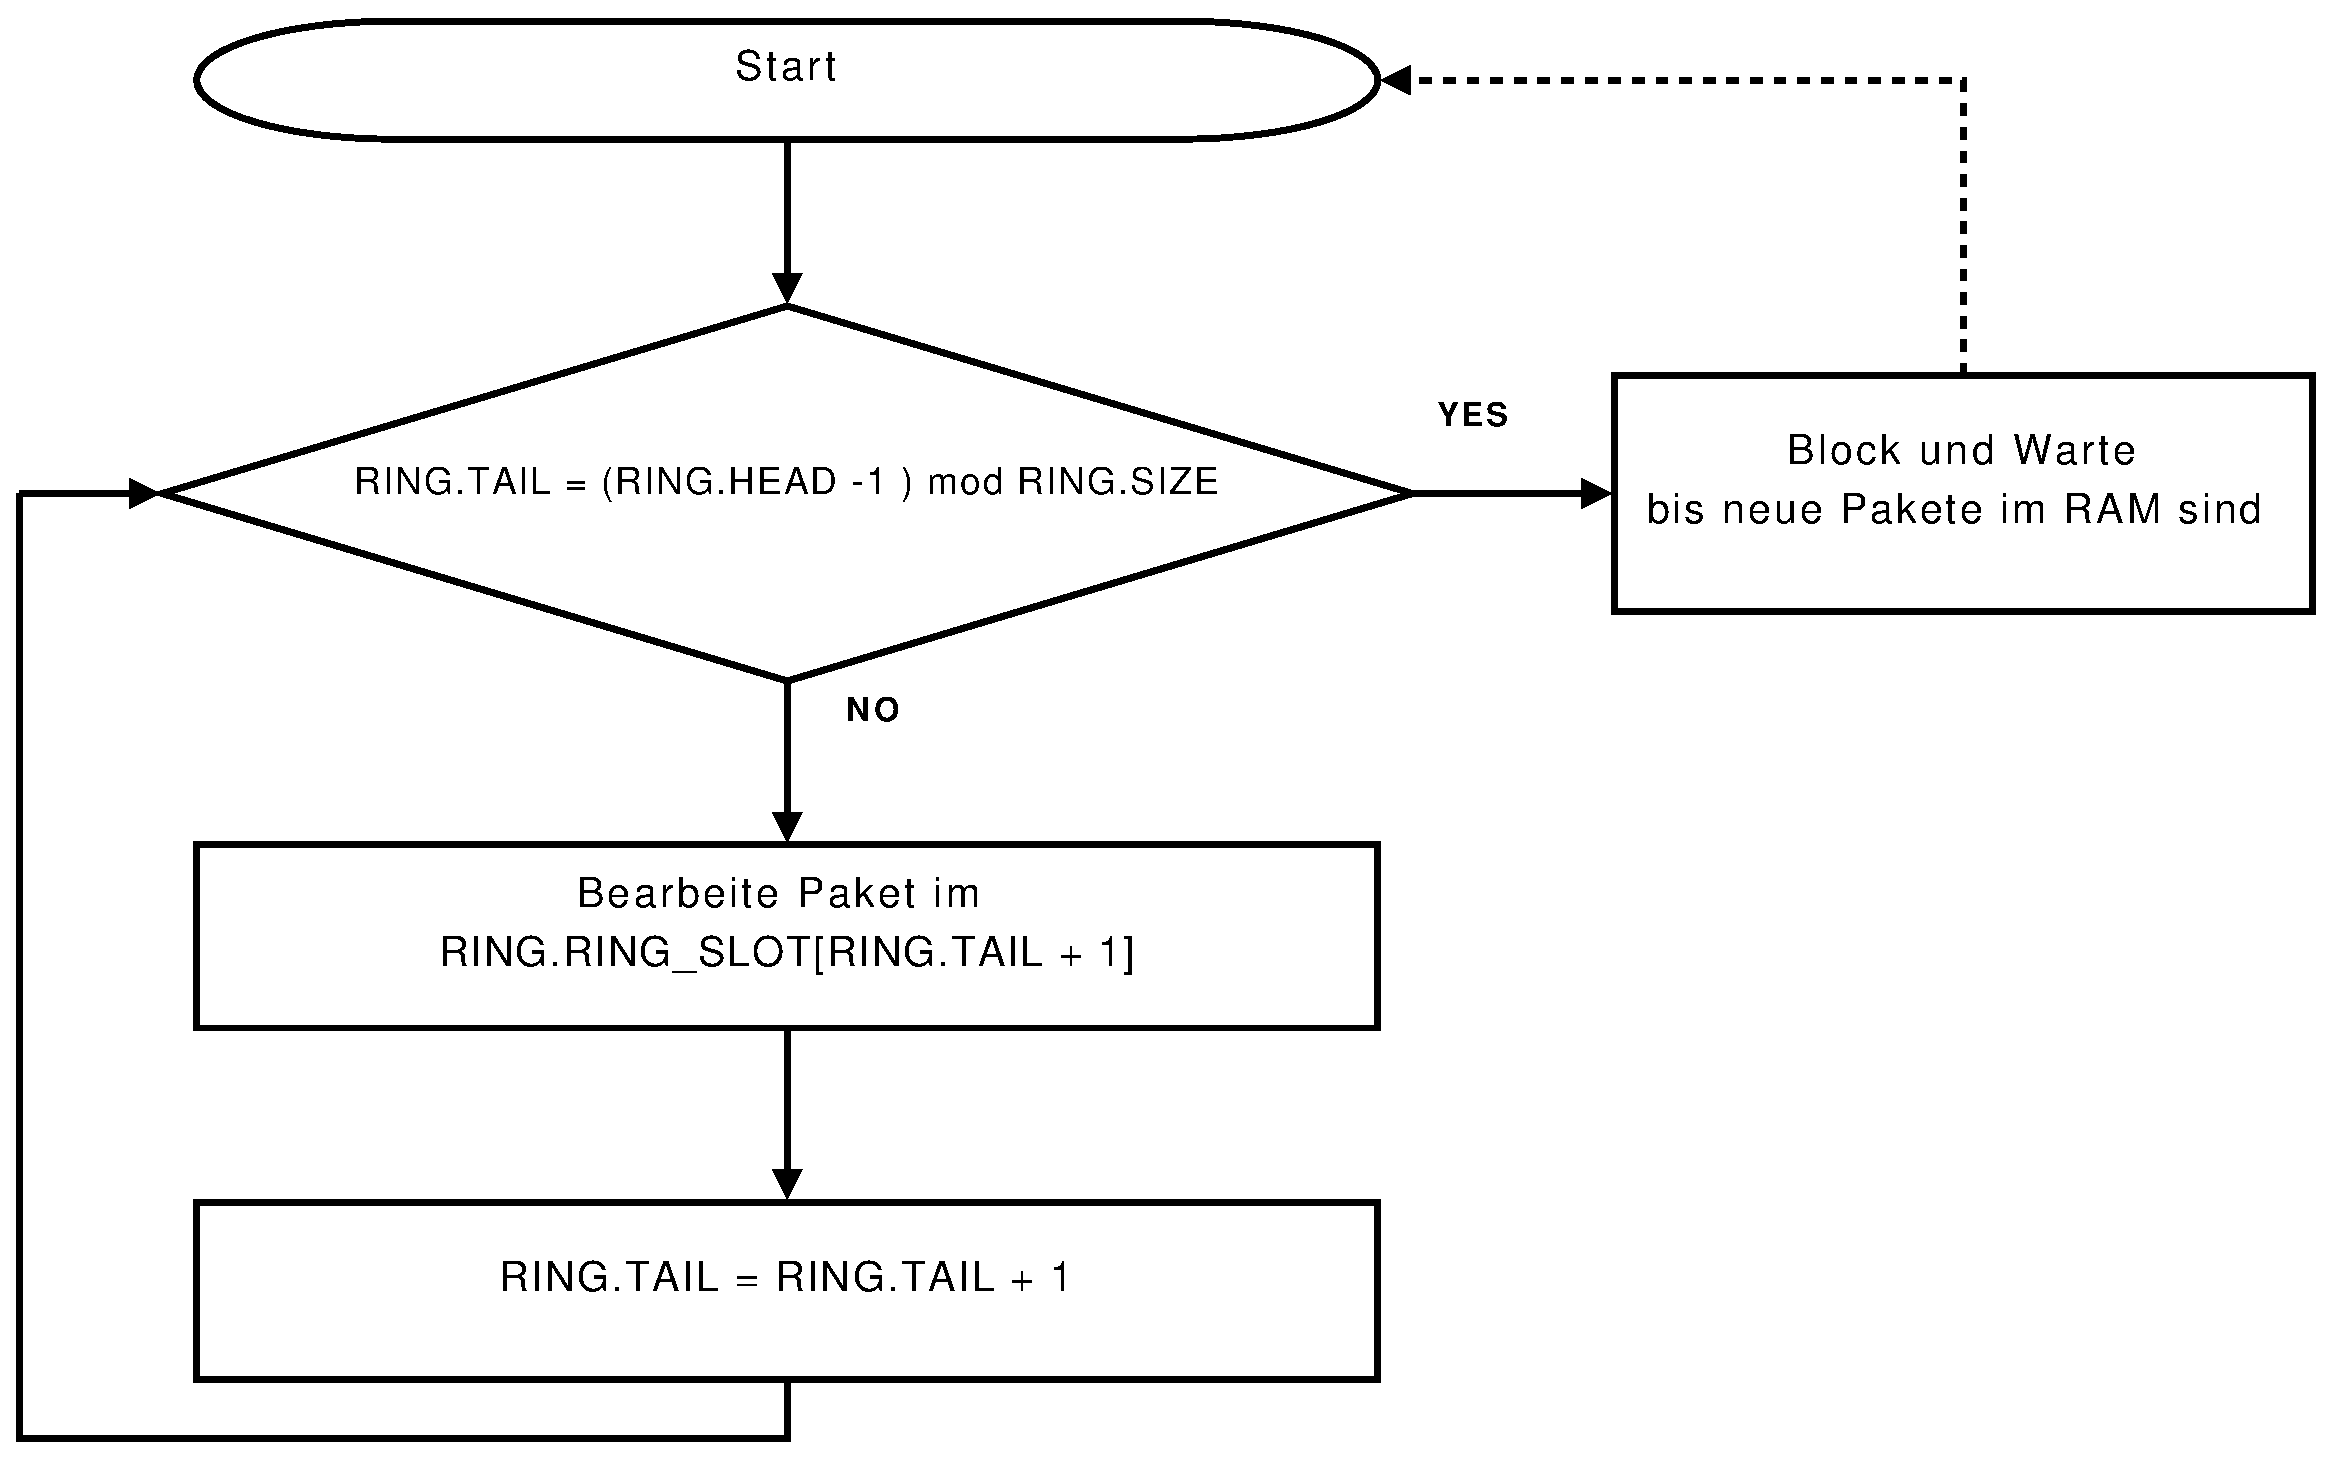
\includegraphics[width=6.0in]{bilder/FlowChart_US_CAP}
\caption{User-Prozess. Capturing-Ablauf}
\label{img:us_capt}
\end{figure}
In Abbildung \ref{img:us_capt} ist der Ablauf des Capturing
in Userspace dargestellt. Der Userspace-Capturing-Prozess liest die \verb+RING_SLOT+'s in der \verb+RING+-Struktur 
der Reihe nach. Nimmt aus den Slots die benötigte Adresse der Paket-Puffer, \verb+mbuf+'s, 
Deskriptoren, und danach bearbeitet bzw. filtert die Pakete, die in den Paket-Puffer
enthalten sind. Beim Bearbeiten jedes Paketes beschreibt der Capturing-Prozess
den \verb+RING.TAIL+ mit der Nummer des gerade gelesenen Paket-Puffer. Sobald 
der \verb+RING.TAIL+ den \verb+RING.HEAD+ nachgeholt hat, was die Abwesenheit 
von neuen Paketen im RAM bedeutet, wird der Prozess blockiert. Sobald die 
neue Pakete in den RAM ankommen, wird nach der Interruptbehandlung der Prozess 
wieder erweckt. \\\\
%
Dadurch, dass der Userspace-Capturing-Prozess sowohl die Paket-Puffer als auch
die \verb+mbuf+'s und Deskriptoren in seinem virtuellen Speicher hat, kann er
aufwendige Paket-Bearbeitung machen. Über die Deskriptor-Felder ist jetzt dem
Userspace-Prozess unterschiedliche Details, die der Netzwerkadapter zur Verfügung
stellt (\verb+Checksum, Lenght, Error+, etc\ldots ) bekannt. Das heißt, man braucht 
keine CPU-Lästige Systemaufrufe um den Zugriff auf die Informationen zu bekommen.

\subsection{Zusammenfassung}
In diesem Kapitel wurde den Entwurf des neuen ringmap-Paket-Capturing-Stack
vorgestellt.  Die Funktionen des Stacks sind für \emph{Paketzustellung},
\emph{Paketzugriff} und \emph{Capturing-Steuerung} zuständig. Die Zustellung-
und Zugriff-Prozess benutzen gemeinsam mehrere Speicher-Bereiche
(\emph{shared-Memory}), die mit Hilfe der \verb+RING+-Struktur in Form eines
Ringpuffers modelliert sind.  Die \verb+RING+-Struktur und  die für
Paketempfang verantwortliche Paket-Puffer sind in Adressraum sowohl des
Zustellung-Prozesses als auch des Zugriff-Prozesses eingeblendet. Dies
ermöglicht den Paketzugriff ohne das teure Kopieren und ohne Systemaufrufe.\\\\
%
Der Zustellung-Prozess wird im Kernelspace und der Zugriff-Prozess im Userspace
ausgeführt. Aufgrund dass es nur einen Zustellung-Prozess und nur einen
Zugriff-Prozess gibt entstehen keine \emph{race conditions}. Deshalb werden
Synchronisation-Massnahmen benötigt.\\\\
%
Für den Zugriffsprozess ist die Funktionalität entworfen, die es ihm erlaubt im
blockierten Zustand auf die neue Pakete zu warten, das Capturing anzuhalten und
wieder fortzusetzen und die Einblendung der für Paketempfang verantwortlichen
Speicherbereichen zu initiieren. Diese Funktionalität soll im Kernelspace
ausführbar sein und dadurch über die Systemaufrufe zur Verfügung stehen.\\\\
Die Implementierungsdetails des Entwurfes sind im folgenden Kapitel
dargestellt.
